\section{Process Perspective}\label{process-perspective}

\subsection{CI/CD Pipelines}\label{cicd-pipelines}
\textit{marho@itu.dk} \\

The CI/CD pipeline consists of three GitHub Action workflows, which can be seen in
\code{/.github/workflows/}. All workflows are run on
\code{ubuntu-24.04}. The first part of our CI pipeline (Build and test workflow) runs on pull-request to main. 
The whole pipeline is run on push to main. 
The following section will give a description of each workflow and how a feature goes to production. This is also illustrated in (FIGURE)
%TODO: Which standard does this diagram follow?
%TODO split up diagram
%TODO fix: maybe building the artefact is actually considered CI?



\pumlfile{cicd.puml}

\subsubsection{Build and test}\label{build-and-test}

The first part of our CI pipeline (Build and Test workflow) consists of the following steps that run in parrallel: 
\begin{enumerate}
    \item \textbf{Code formatter with Csharpier}: Checks the layout of the code. 
    This helps ensure that the layout is alike thoughout the codebase. It does not automaticly apply layout changes, but reports it back on GitHub.
    \item \textbf{Dockerfile linter with Hadolint}: Lints the MiniTwit dockerfile.
    \item \textbf{Build the application}: Builds the applications and:
    \begin{itemize}
        \item Run unit and intergreation tests
        \item Run tests on the API / simulator endpoint.
        \item Runs E2E / Playwright tests
    \end{itemize}
\end{enumerate}

\subsubsection{CI/CD}
The CI/CD workflow runs on a succesfull Build and Test workflow and push to main. It consists of the following steps that run sequentially:
\begin{enumerate}
    \item \textbf{Dockerhub}:
    \begin{itemize}
        \item Github Actions builds and pushes the \code{Minitwit}, \code{Grafana}, \code{Alloy}, \code{Loki} and \code{Prometheus} docker images to Dockerhub.
    \end{itemize}
    \item \textbf{SSH and Deploy}
    \begin{itemize}
        \item SSH into the node named leader in the swarm.
        \item Copy the stack file \path{/itu-minitwit/infrastructure/docker_swarm/stack/minitwit_stack.yml} to the node.
        \item Deploy to the swarm.
    \end{itemize}
\end{enumerate}

\subsubsection{Release}\label{release}

The release workflow runs on a successfull CI/CD run. It builds and zips
the application for Windows, Mac and Linux.

\subsubsection{SonarQube}\label{sonarqube}
\textit{Morten}
SonarQube runs on pull requests as a step in our CI pipeline. It checks for security issues, code smells and the quality of the code.
SonarQube also gives a Quality Gate, that fails if the threshold for the pull-request is too low 
e.g. Security, Reliability and Maintainability.
SonarQube is not blocking 
meaning we could still merge, even if SonarQube fails, it more used as a reminder of better coding practices and 
error handling.   

\subsection{Monitoring}\label{monitoring}
\textit{marho@itu.dk} \\

The system uses Prometheus for monitoring. 
Prometheus scrapes the \code{/metrics} endpoint on each MiniTwit service instance.
Grafana then queries Prometheus, which displays and visualises the data. 
Monitoring is done on a business level, application level, and infrastructure level.
The monitoring setup can be seen in figure \ref{mon-diagram}

\subsubsection{Business monitoring}\label{business-monitoring}

On a business level we monitor:
\begin{itemize}
    \item Number of created accounts
    \item Average follower count per user
    \item Total number of cheeps over time
\end{itemize}

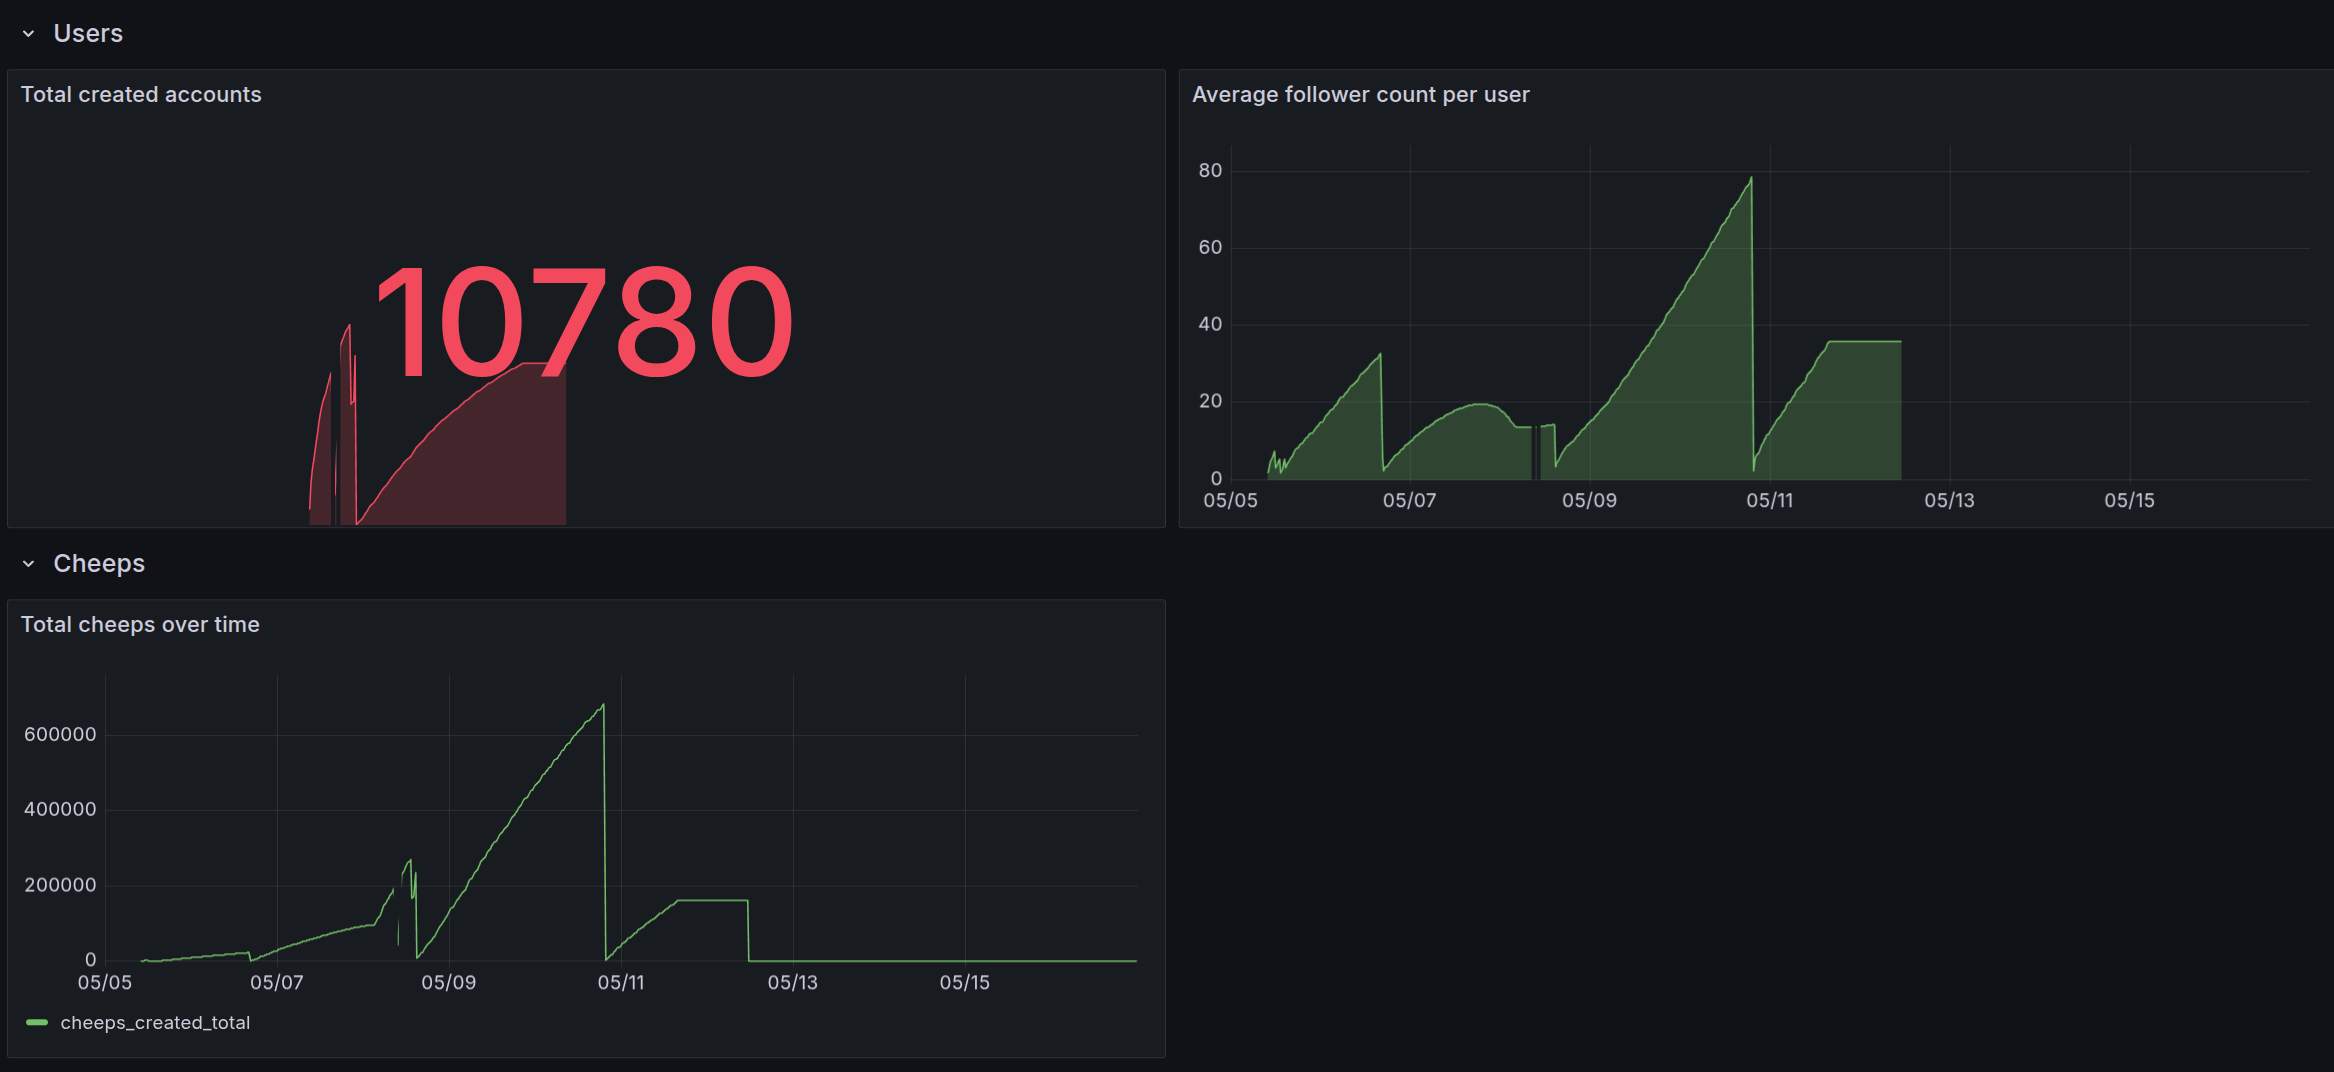
\includegraphics[width=\textwidth]{images/monitoring_business.png}

\subsubsection{Application monitoring}\label{application-monitoring}

On an application level we monitor the durations of different database queries that
MiniTwit makes:
\begin{itemize}
    \item GetCheeps - Gets cheeps for a given page
    \item GetCheepsFromAuthor - Getting an Authors cheeps
    \item AddCheep - Create a cheep
\end{itemize}

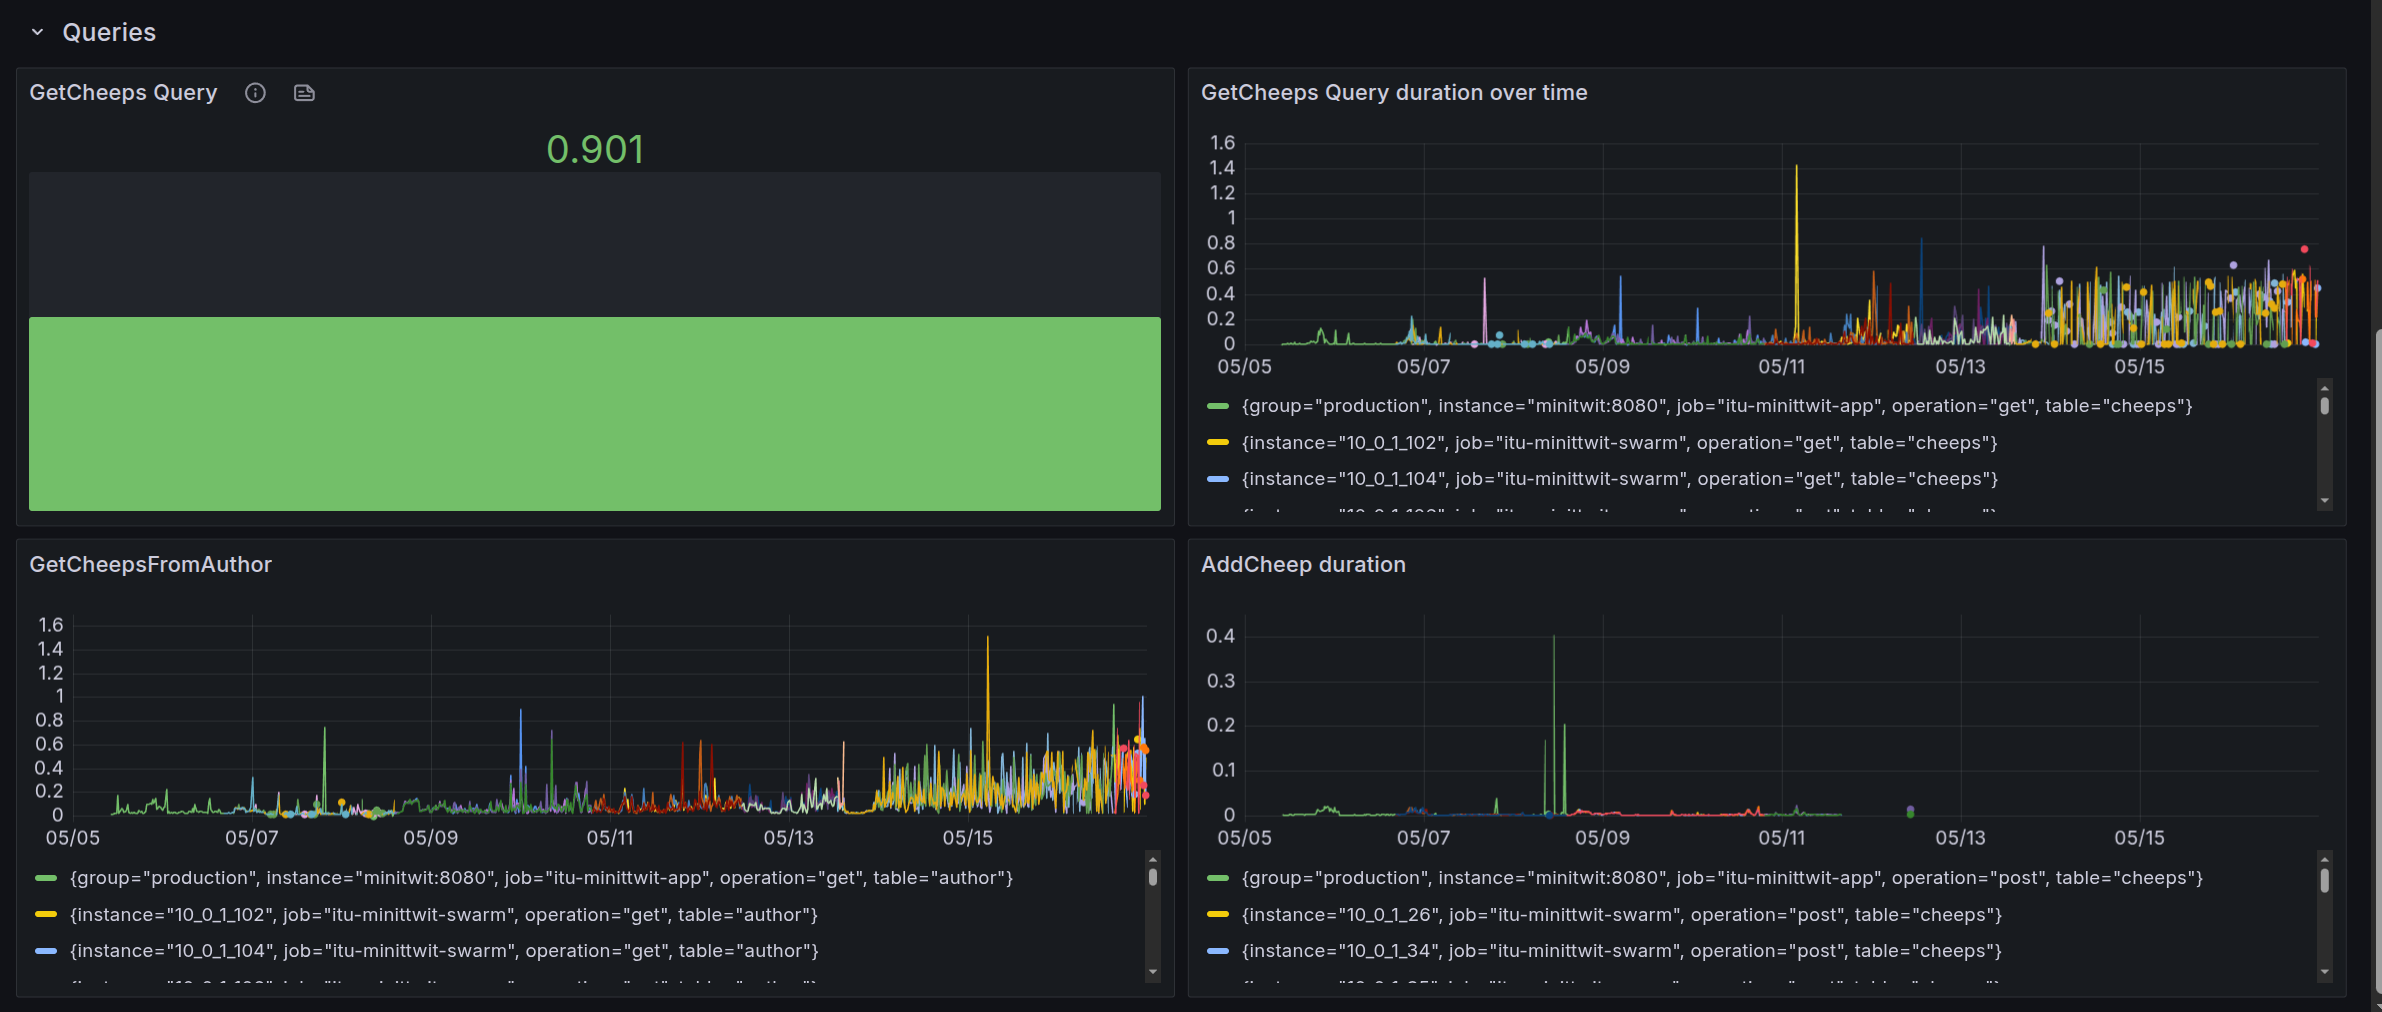
\includegraphics[width=\textwidth]{./images/monitoring_queries.png}

\subsubsection{Infrastructure
monitoring}\label{infrastructure-monitoring}

On an infrastructure level we monitor:
\begin{itemize}
    \item The status of nodes
    \item Memory usage of nodes
    \item CPU usage of nodes
    \item HTTP requests per minute for each node
\end{itemize}

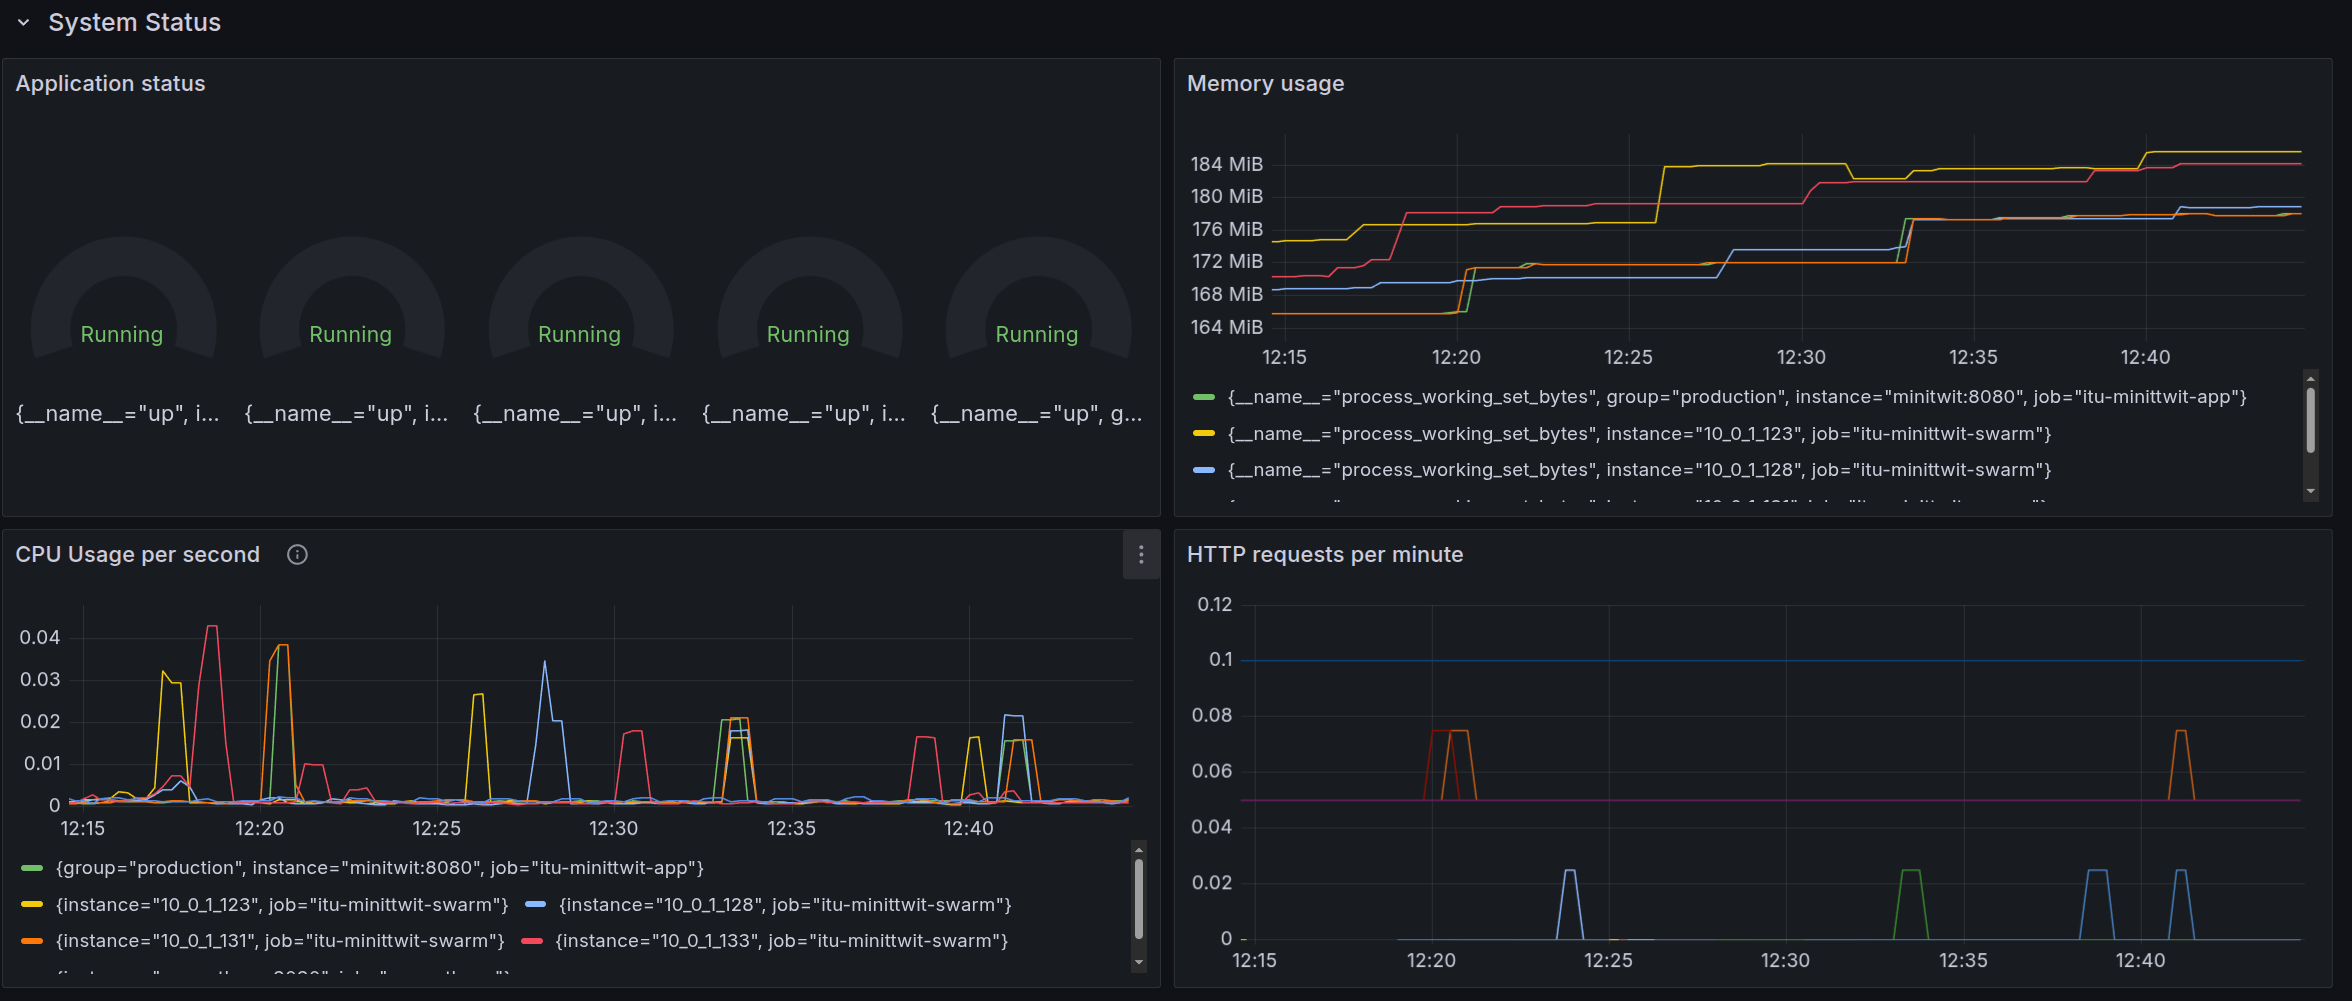
\includegraphics[width=\textwidth]{./images/system_status.png}

\subsection{Logging}\label{processlogging}
\textit{Marius} \\

The application uses a Grafana-loki-alloy stack to log all services. The logging setup can be seen in figure \ref{mon-diagram}

\subsubsection{What we log}\label{what-we-log}
We currently log the logs from each docker service, as described in our 
\code{/infrastructure/docker\_swarm/stack/minitwit\_stack.yml} file. As will be discussed in \ref{importance-of-good-logging}, 
more comprehensive logging would have been beneficial.


\subsubsection{Aggregation of logs}\label{aggregation-of-logs}
We use Alloy to push logs from each node to Loki, which collects them. The logs are displayed on grafana, which can
be seen in the logging dashboard:

\begin{figure} [H]
    \pumlfile{monitoring.puml}
    \caption{Deployment diagram of the monitoring and logging setup}
    \label{mon-diagram}
\end{figure}

\begin{figure}[H]
\centering
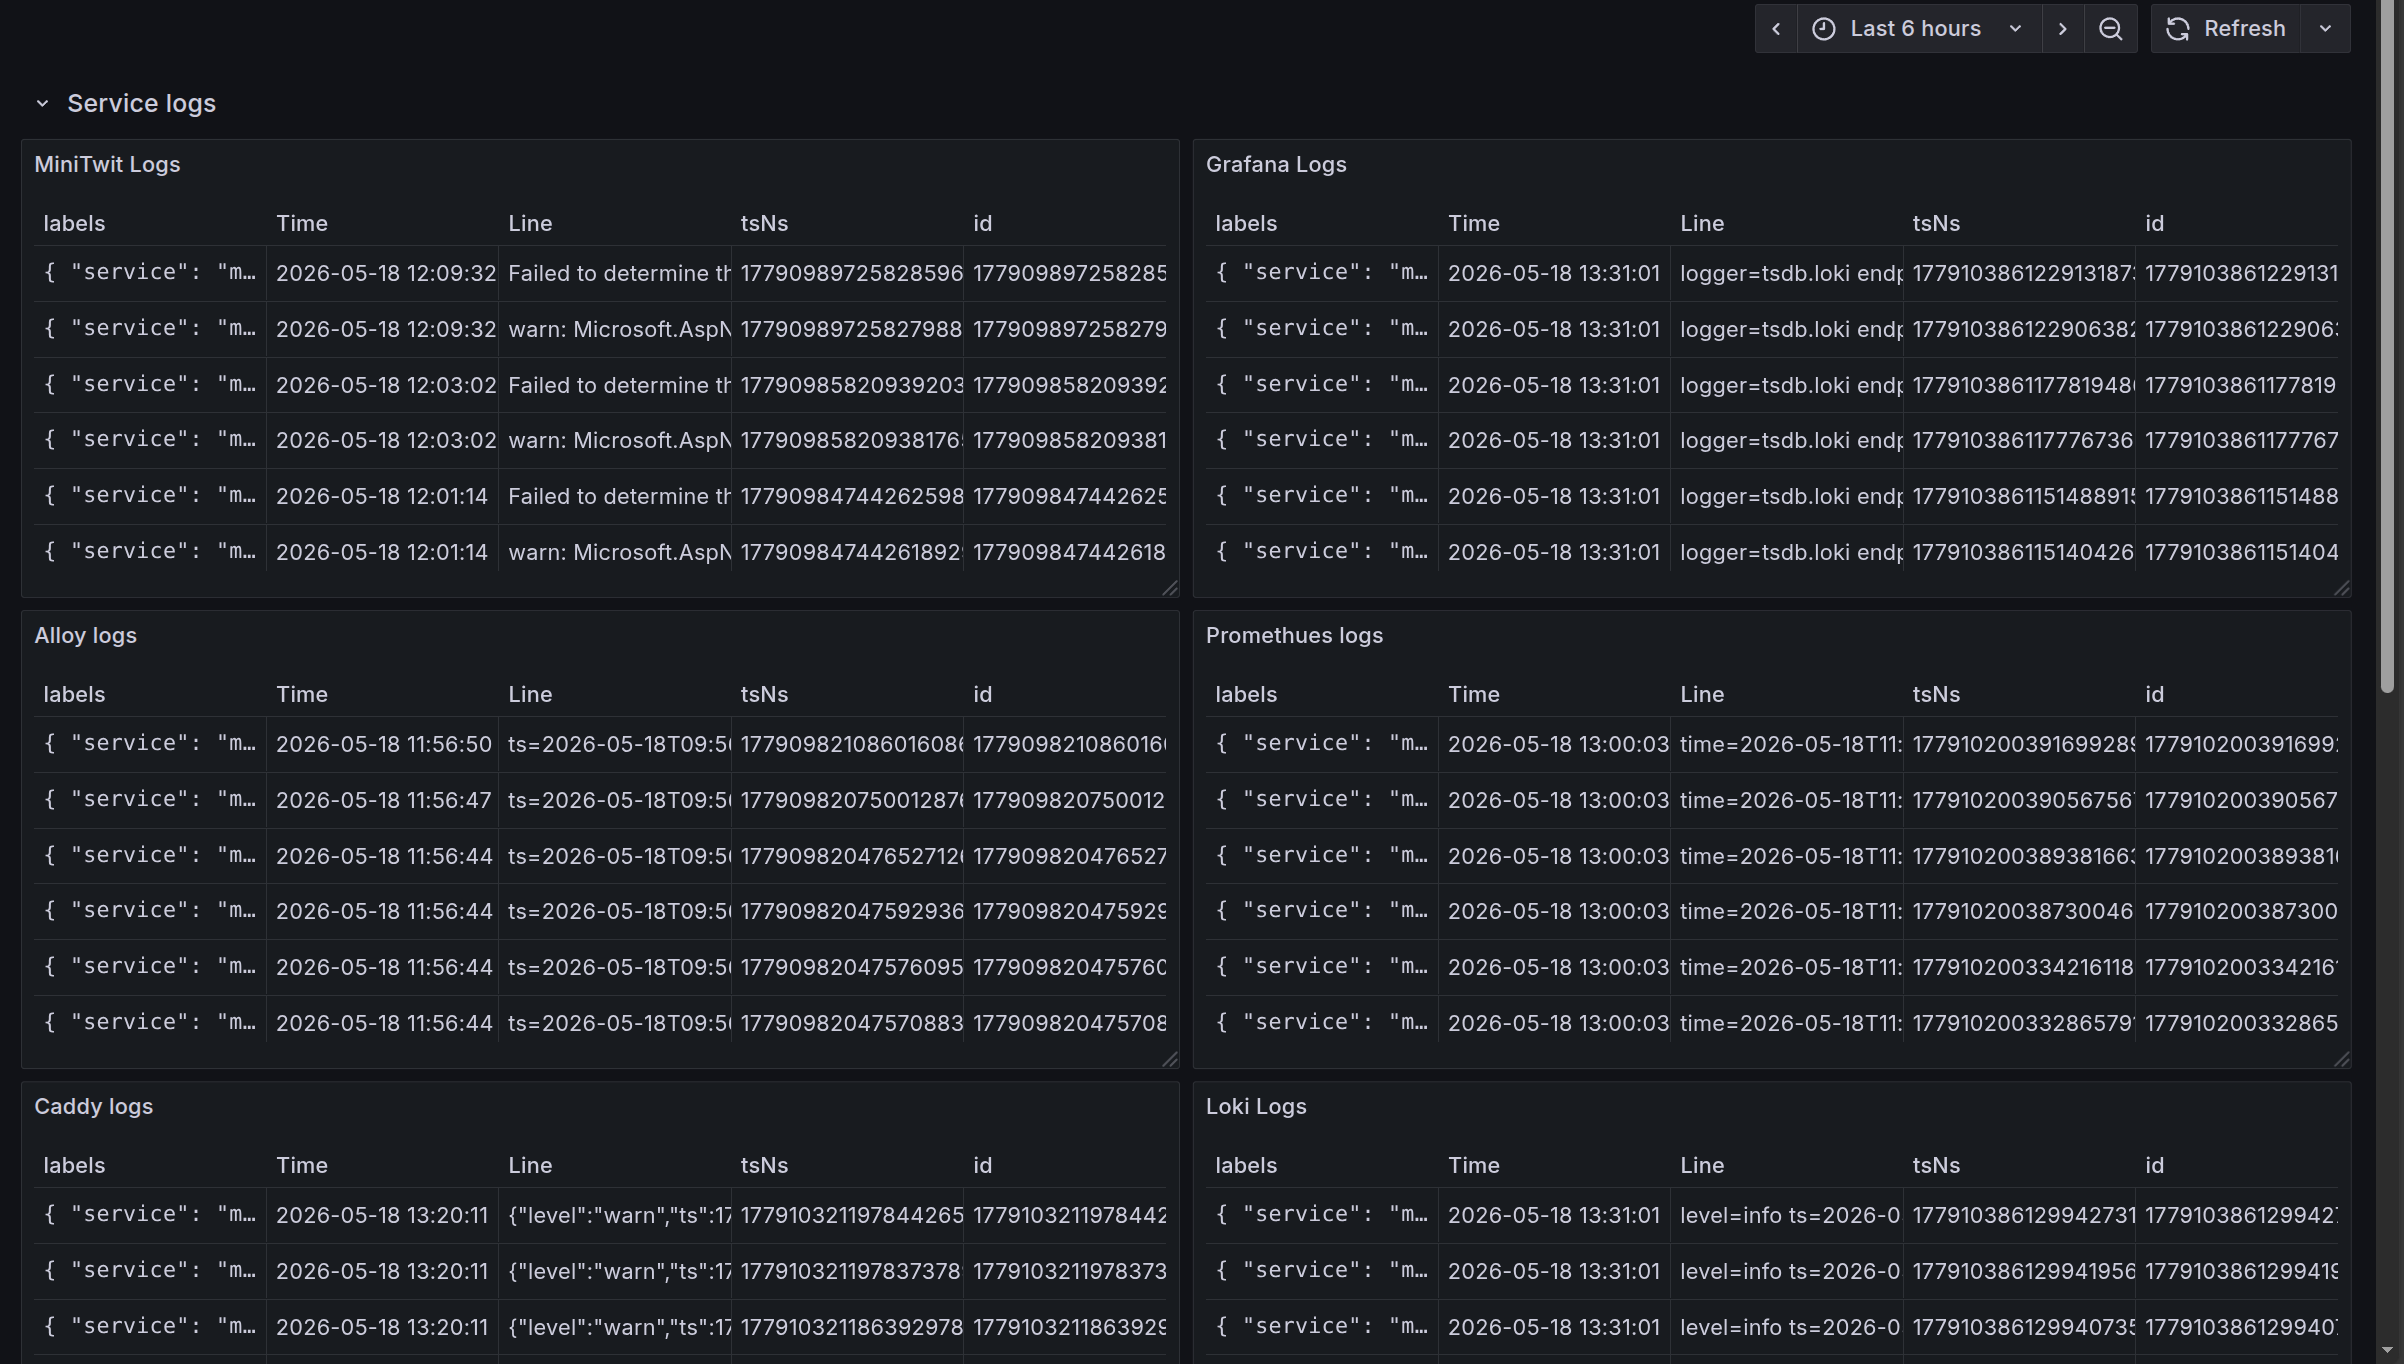
\includegraphics[width=\textwidth]{./images/logging_dashboard.png}
\caption{logging\_dashboard}
\end{figure}

\subsection{Security hardening}\label{security-hardening}
\textit{Jonas} 

To protect against supply line attacks, we would select docker hardened images from \url{dhi.io} to use for our dependencies; Prometheus, Alloy, Loki, Grafana.
We would also go through our Minitwit application and adjust it to comply with the rules at \url{https://cheatsheetseries.owasp.org/cheatsheets/Docker_Security_Cheat_Sheet.html}.
However, we did not manage to fully implement this, so it is not used in produciton.

\subsection{Availability and scaling}\label{availability-and-scaling}
\textit{Marius \& Morten} \\

To scale and ensure availability of the application Terraform and Docker
Swarm is used.

\subsubsection{Availability}\label{availability}
The application consists of five nodes that are a part of a swarm
cluster, 2 workers, 2 managers and 1 leader, that together run four replicated minitwit services.
All nodes run Alloy.
The ``Leader'' node also runs Caddy, Grafana, Prometheus and Loki.
Figure \ref{deployment-diagram} illustrates this.
\sloppy See
\code{terraform/minitwit\_swarm\_cluster.tf} and
\code{docker\_swarm/stack/minitwit\_stack.yml} under
\code{/infrastructure} for the code. Having multiple services running MiniTwit ensures that even if a docker service or swarm node
fails, the application is still available.

\textbf{Single Point of Failure}: Multiple services like Caddy and Grafana are pinned to the ``Leader'' node. This creates SPOF for those services. 
As we only have one Caddy load balancer service,
living on the ``Leader'' node, that takes HTTPS requests on our
\code{devbobs.tech} domain. This is a single point of failure for
accessing the application from \code{devbobs.tech} and using HTTPS. If
the ``Leader'' node goes down, it is still possible to access the other nodes
IPs on port :8080 without HTTPS. The docker ingress routing mesh
will in that case take care of load balancing, instead of Caddy.

\subsubsection{Scaling}\label{scaling}

The application can be scaled in two different ways: \textbf{Vertical
scaling}: A single node can be scaled vertically either by rezising the
node in DigitalOcean or changing the \code{size} field in
\code{minitwit\_swarm\_cluster.tf} and applying it with terraform.
\textbf{Horizontal scaling}: The deployment of the application can be
scaled horizontal by increasing the amount of nodes in the cluster. This
can be done by increasing the \code{count} number of e.g.~a Worker
node and then make it join the swarm, by running the \code{bootstrap.sh} script 
again, which apply the change with terraform.
Horizontal scaling can also be achieved by increasing the amount of minitwit instances per node, increasing redundancy.
When scaling horisontally the load balancer distributes the requests.
